%%=============================================================================
%% Resultaten
%%=============================================================================

\chapter{\IfLanguageName{dutch}{Resultaten en evaluatie}{Resultaten en evaluatie}}%
\label{ch:resultaten}

Dit hoofdstuk bespreekt de resultaten van de uitgevoerde evaluatie van de drie AI-varianten binnen DepGuard AI. De analyse vertrekt vanuit de benchmarkuitvoer van de proof-of-concept en vergelijkt de oplossingen op het vlak van specificiteit, volledigheid, actiegerichtheid en verwerkingstijd. Op basis daarvan wordt nagegaan in welke mate de verschillende benaderingen bruikbare ondersteuning bieden voor dependencybeheer in de context van Springbok.

\section{Evaluatiekader}
\label{sec:evaluatiekader}

Vooraleer de resultaten worden besproken, wordt in deze sectie toegelicht hoe de evaluatie is opgezet. Eerst wordt de gebruikte scoremethode -- \textit{LLM-as-a-Judge} -- beschreven, inclusief de beoordelingsdimensies, gewichten en scoringsformules. Daarna worden de vijf testcases geïntroduceerd en gemotiveerd, met per testcase een overzicht van de verwachte output op basis van de officiële changelog.

\subsection{Scoremethode: LLM-as-a-Judge}
\label{subsec:scoremethode}

Om de output van de drie AI-agents op een consistente en herhaalbare manier te beoordelen, maakt de benchmark gebruik van de \textit{LLM-as-a-Judge}-aanpak. Bij deze evaluatiemethode treedt een tweede taalmodel op als rechter en beoordeelt de output van de agent semantisch, zonder te vertrekken van vaste regelsets of eenvoudige keyword-matching. De judge begrijpt de \textit{betekenis} van de output en vergelijkt die inhoudelijk met de verwachte kwaliteit en feiten. Dit is precies wat LLM-as-a-Judge onderscheidt van klassieke evaluatiemethodes.

In deze benchmark is het judge-model \texttt{gpt-4o-mini}, geconfigureerd met een lage temperatuur (\texttt{temperature=0.1}) om consistente en herhaalbare oordelen te garanderen. Elke agent-output wordt beoordeeld op vier kwantitatieve dimensies (schaal 0--10) en twee kwalitatieve indicatoren:

\begin{enumerate}
    \item \textbf{Specificiteit} (30\,\% gewicht): meet of de analyse concrete, package-specifieke informatie bevat. Lage scores wijzen op vage of generieke tekst; hoge scores impliceren exacte API-namen, versienummers of codefragmenten.
    \item \textbf{Actiegerichtheid} (40\,\% gewicht): meet of een developer op basis van deze output een gefundeerde beslissing kan nemen over de update, zonder zelf de changelog te raadplegen. Dit is de zwaarst wegende dimensie, omdat het de kernvraag van het systeem beantwoordt.
    \item \textbf{Volledigheid} (15\,\% gewicht): meet of alle verwachte secties aanwezig zijn: nieuwe functies, breaking changes, migratiestappen en een expliciete veiligheidsinschatting.
    \item \textbf{Feitendekking} (15\,\% gewicht): meet hoeveel van de vooraf gedefinieerde verwachte feiten (\textit{expected facts}) de agent correct en volledig vermeldt. Hiermee wordt de output getoetst aan de grondwaarheid uit de officiële changelog.
\end{enumerate}

De overall score per run wordt berekend als gewogen gemiddelde:
\begin{equation}
    \text{overall} = \text{actiegerichtheid} \times 0{,}40
                   + \text{specificiteit} \times 0{,}30
                   + \text{volledigheid} \times 0{,}15
                   + \text{feitendekking} \times 0{,}15
    \label{eq:overallscore}
\end{equation}

Naast de vier dimensies detecteert de judge ook twee booleaanse indicatoren en een categorisch veiligheidsoordeel (\textit{Yes}, \textit{No}, \textit{With caution} of \textit{Not found}). Elk testgeval wordt driemaal uitgevoerd per agent, waarna de gerapporteerde scores de rekenkundige gemiddelden zijn over die drie runs. De consistentiescore meet de stabiliteit van een agent over deze herhalingen:

\begin{equation}
    \text{consistentie} = \max\bigl(0,\; 10 - \sigma_{\text{overall}} \times 2\bigr)
    \label{eq:consistentie}
\end{equation}

waarbij $\sigma_{\text{overall}}$ de standaardafwijking is van de overallscores. Een agent die sterk varieert tussen runs scoort lager op consistentie en is in productie minder betrouwbaar.

\subsection{Testcaseselectie en verwachte output}
\label{subsec:testcases}

De benchmark omvat vijf testcases die samen de volledige breedte van updatetypes -- \textit{patch}, \textit{minor} en \textit{major} -- dekken, verspreid over uiteenlopende packagecategorieën en risiconiveaus. De selectie is als volgt gemotiveerd:

\begin{itemize}
    \item \textbf{react minor (18.2.0 → 18.3.0):} React is een van de meest gebruikte frontend bibliotheken en een frequent terugkerende dependency in projecten zoals die van Springbok. Deze minor update voegt functioneel niets toe maar introduceert uitsluitend deprecatiewaarschuwingen voor React 19. Het is daarmee een \textit{edge case}: agents die de update simpelweg als ``veilig zonder bijzonderheden'' beschrijven missen essentiële informatie voor toekomstgericht onderhoud.
    \item \textbf{next.js minor (14.1.0 → 14.2.0):} Next.js is een veelgebruikte meta-framework in productieomgevingen. Deze minor update brengt aanzienlijke prestatie- en stabiliteitsverbeteringen met zich mee (Turbopack, geheugenverbruik). Agents worden getest op hun vermogen om niet-triviale verborgen meerwaarde te herkennen en te rapporteren.
    \item \textbf{TypeScript major (4.9.5 → 5.0.4):} Een major update met reële breaking changes (nieuwe decoratorstandaard, deprecated tsconfig-opties, gewijzigde minimumversies). Dit is de moeilijkste testcase en meet de kwaliteit van risicoanalyse bij updates met hoge impact.
    \item \textbf{zod patch (3.22.3 → 3.22.4):} Een patch binnen een stabiele minor-lijn waarvoor de officiële changelog geen gedetailleerde patchnotes publiceert. Dit dient als \textit{eerlijkheidstest}: een betrouwbare agent vermeldt dat specifieke details niet beschikbaar zijn, in plaats van concrete bugfixes te verzinnen.
    \item \textbf{tailwindcss minor (3.3.0 → 3.4.0):} Een minor update met uitgebreide nieuwe utilities (dynamische viewport-eenheden, \texttt{has-*}-variant, \texttt{size-*}-utilities, subgrid) die volledig backwards compatibel zijn. Agents worden getest op hun vermogen om een brede set nieuwe functies correct en volledig te rapporteren.
\end{itemize}

De vijf testcases bestrijken samen drie risiconiveaus (patch, minor, major), vijf packagedomeinen (UI-framework, meta-framework, typesysteem, validatiebibliotheek, CSS-framework) en twee bijzondere scenario's (deprecaties zonder breaking changes; patch zonder publieke notes). Tabel~\ref{tab:testcases} vat de details samen.

\begin{table}[h]
    \centering
    \caption{Overzicht van de gebruikte testcases met verwacht veiligheidsoordeel}
    \label{tab:testcases}
    \begin{tabular}{llllp{5.5cm}}
        \hline
        \textbf{ID} & \textbf{Package} & \textbf{Versieovergang} & \textbf{Type} & \textbf{Verwacht oordeel \& kernpunten} \\
        \hline
        react\_minor       & react       & 18.2.0 → 18.3.0 & minor & \textit{Yes} — alleen deprecatiewaarschuwingen; geen nieuwe functies \\
        nextjs\_minor      & next        & 14.1.0 → 14.2.0 & minor & \textit{Yes} — Turbopack-verbeteringen, drastische geheugenreductie \\
        typescript\_major  & typescript  & 4.9.5 → 5.0.4   & major & \textit{With caution} — nieuwe decorators, deprecated tsconfig-opties \\
        zod\_patch         & zod         & 3.22.3 → 3.22.4 & patch & \textit{Yes} — geen publieke patchnotes; eerlijkheidstest \\
        tailwind\_minor    & tailwindcss & 3.3.0 → 3.4.0   & minor & \textit{Yes} — uitgebreide nieuwe utilities, volledig compatibel \\
        \hline
    \end{tabular}
\end{table}

\section{Globale resultaten}
\label{sec:globale-resultaten}

De benchmark werd uitgevoerd op 17 mei 2026 en omvat in totaal 45 evaluaties: 5 testcases $\times$ 3 agents $\times$ 3 runs. Alle gerapporteerde scores zijn rekenkundige gemiddelden over de drie runs. Tabel~\ref{tab:benchmarkresultaten} vat de geaggregeerde resultaten samen per variant.

\begin{table}[h]
    \centering
    \caption{Samenvatting van de benchmarkresultaten per AI-variant (gemiddelden over 5 testcases $\times$ 3 runs)}
    \label{tab:benchmarkresultaten}
    \begin{tabular}{lccccc}
        \hline
        \textbf{Variant} & \textbf{Overall} & \textbf{Specificiteit} & \textbf{Volledigheid} & \textbf{Actiegerichtheid} & \textbf{Gem.\ latency} \\
        \hline
        Mastra  & 7,81          & 7,27          & 8,20          & 8,27          & 10,94~s \\
        OpenAI  & 6,53          & 5,60          & 8,00          & 7,27          & 4,34~s \\
        n8n     & 6,04          & 4,67          & 6,67          & 7,47          & 8,07~s  \\
        \hline
    \end{tabular}
\end{table}

Figuur~\ref{fig:scores-per-testcase} toont de overallscores per testcase en per agent. Hieruit blijkt dat de drie varianten sterk uiteenlopen naargelang het type update, en dat geen enkele variant in alle testcases dominant is.

\begin{figure}[H]
    \centering
    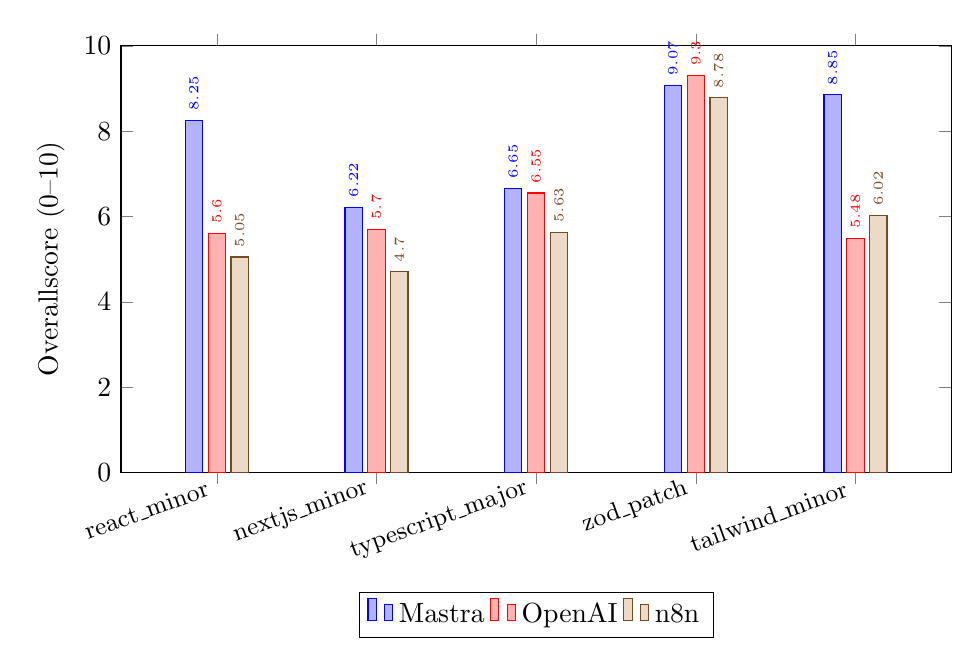
\begin{tikzpicture}
        \begin{axis}[
            ybar,
            bar width=0.22cm,
            width=\linewidth,
            height=7cm,
            ymin=0, ymax=10,
            ylabel={Overallscore (0--10)},
            xtick=data,
            symbolic x coords={react\_minor, nextjs\_minor, typescript\_major, zod\_patch, tailwind\_minor},
            xticklabel style={rotate=20, anchor=east, font=\small},
            legend style={at={(0.5,-0.28)}, anchor=north, legend columns=3},
            nodes near coords,
            nodes near coords style={font=\tiny},
            every node near coord/.append style={rotate=90, anchor=west},
            enlarge x limits=0.15,
        ]
        \addplot coordinates {
            (react\_minor, 8.25)
            (nextjs\_minor, 6.22)
            (typescript\_major, 6.65)
            (zod\_patch, 9.07)
            (tailwind\_minor, 8.85)
        };
        \addplot coordinates {
            (react\_minor, 5.60)
            (nextjs\_minor, 5.70)
            (typescript\_major, 6.55)
            (zod\_patch, 9.30)
            (tailwind\_minor, 5.48)
        };
        \addplot coordinates {
            (react\_minor, 5.05)
            (nextjs\_minor, 4.70)
            (typescript\_major, 5.63)
            (zod\_patch, 8.78)
            (tailwind\_minor, 6.02)
        };
        \legend{Mastra, OpenAI, n8n}
        \end{axis}
    \end{tikzpicture}
    \caption{Gemiddelde overallscores per testcase en per agent (gemiddeld over 3 runs)}
    \label{fig:scores-per-testcase}
\end{figure}
\FloatBarrier

Figuur~\ref{fig:dimensies-per-agent} vergelijkt de gemiddelde scores per beoordelingsdimensie over alle testcases.
 
\begin{figure}[H]
    \centering
    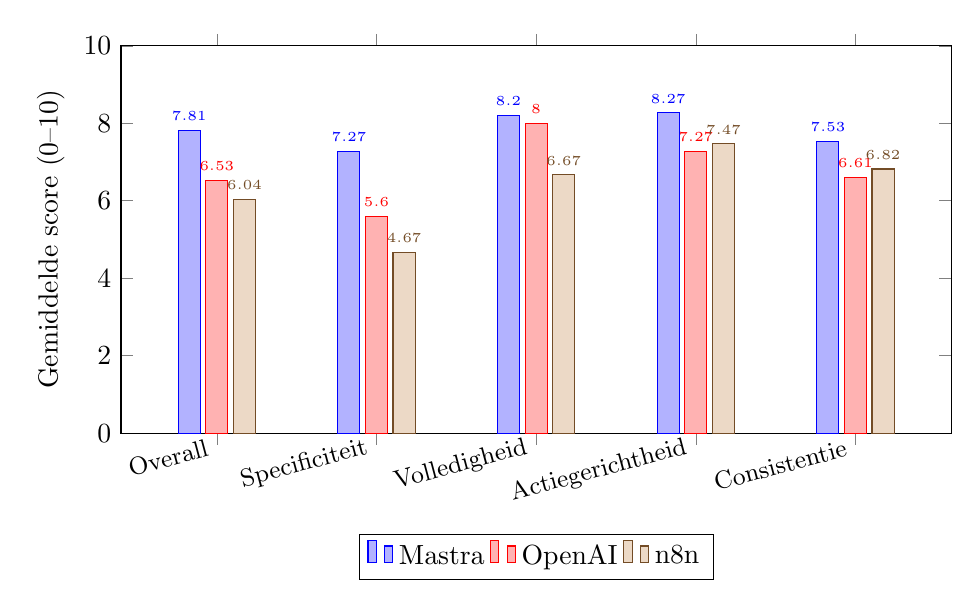
\begin{tikzpicture}
        \begin{axis}[
            ybar,
            bar width=0.28cm,
            width=\linewidth,
            height=6.5cm,
            ymin=0, ymax=10,
            ylabel={Gemiddelde score (0--10)},
            xtick=data,
            symbolic x coords={Overall, Specificiteit, Volledigheid, Actiegerichtheid, Consistentie},
            xticklabel style={rotate=15, anchor=east, font=\small},
            legend style={at={(0.5,-0.26)}, anchor=north, legend columns=3},
            nodes near coords,
            nodes near coords style={font=\tiny},
            enlarge x limits=0.15,
        ]
        \addplot coordinates {
            (Overall, 7.81)
            (Specificiteit, 7.27)
            (Volledigheid, 8.20)
            (Actiegerichtheid, 8.27)
            (Consistentie, 7.53)
        };
        \addplot coordinates {
            (Overall, 6.53)
            (Specificiteit, 5.60)
            (Volledigheid, 8.00)
            (Actiegerichtheid, 7.27)
            (Consistentie, 6.61)
        };
        \addplot coordinates {
            (Overall, 6.04)
            (Specificiteit, 4.67)
            (Volledigheid, 6.67)
            (Actiegerichtheid, 7.47)
            (Consistentie, 6.82)
        };
        \legend{Mastra, OpenAI, n8n}
        \end{axis}
    \end{tikzpicture}
    \caption{Gemiddelde scores per beoordelingsdimensie over alle testcases}
    \label{fig:dimensies-per-agent}
\end{figure}
\FloatBarrier

Mastra scoort het hoogst op overall (7,81), specificiteit (7,27), volledigheid (8,20) en actiegerichtheid (8,27). De agent haalt ook de hoogste consistentiescore (7,53), wat aangeeft dat de output over meerdere runs stabiel blijft. Het nadeel is de aanzienlijk hogere latency: gemiddeld 10,94\,s tegenover 4,34\,s voor OpenAI. OpenAI scoort beduidend lager op specificiteit (5,60) en actiegerichtheid (7,27), maar is de snelste variant. n8n presteert op alle dimensies het laagst, met name op specificiteit (4,67) en volledigheid (6,67).

\section{Analyse per testcase}
\label{sec:analyse-per-testcase}

De vijf testcases worden hieronder afzonderlijk besproken. Per testcase wordt eerst de verwachte output beschreven op basis van de handmatig samengestelde \textit{expected facts} uit de officiële changelog. Daarna worden de scores en de kwalitatieve bevindingen per agent toegelicht, met aandacht voor wat correct werd gerapporteerd, wat ontbrak en waar hallucinaties optraden.

\subsection{React minor (18.2.0 → 18.3.0)}
\label{subsec:tc-react}
 
\textbf{Verwachte output:} de agent dient te vermelden dat deze release functioneel identiek is aan 18.2.0, uitsluitend deprecatiewaarschuwingen toevoegt (o.a. \texttt{ReactDOM.render}, \texttt{ReactDOM.hydrate}, \texttt{defaultProps} op functiecomponenten), en dat de update veilig is.
 
\textbf{Resultaten:} Mastra behaalt een gemiddelde overallscore van 8,25 en scoort het best op deze testcase. De agent identificeert de deprecaties correct en vermeldt dat er geen breaking changes zijn. In twee van drie runs noemt Mastra echter \texttt{findDOMNode} en \texttt{test-utils} als deprecated, wat niet terugkomt in de officiële changelog -- een voorbeeld van lichte hallucinatie. OpenAI scoort gemiddeld 5,60 en verzint in twee van drie runs nieuwe functies die helemaal niet in React 18.3.0 zijn geïntroduceerd (o.a.\ \texttt{useTransition} en \texttt{startTransition}, die al in React 18.0 bestonden). n8n (gem.\ 5,05) geeft in de meeste runs een sjabloonmatige output waarbij alle secties als ``None in this release'' worden ingevuld, waardoor de relevante deprecatieinformatie volledig ontbreekt.

\subsection{Next.js minor (14.1.0 → 14.2.0)}
\label{subsec:tc-nextjs}
 
\textbf{Verwachte output:} de agent dient de Turbopack-stabilisering, de drastische geheugenreductie bij production builds (van $\sim$2,2\,GB naar $<$190\,MB), de verbeterde hydration error messages en het nieuwe \texttt{staleTimes}-configuratieveld te vermelden. Er zijn geen breaking changes.
 
\textbf{Resultaten:} Dit is de moeilijkste minor-testcase, met de laagste scores voor alle drie de agents. Mastra behaalt een gemiddelde overallscore van 6,22, maar hallucineerde in twee runs breaking changes die niet in de changelog voorkomen (o.a.\ de verwijdering van de \texttt{squoosh}-afhankelijkheid). OpenAI scoort gemiddeld 5,70 en vermeldt eveneens incorrecte breaking changes. Beide agents missen de kernboodschap over de geheugenverbetering, die in productie potentieel de meeste waarde heeft. n8n (gem.\ 4,70) geeft de meest oppervlakkige output en mist migratiestappen in twee van drie runs.

\subsection{TypeScript major (4.9.5 → 5.0.4)}
\label{subsec:tc-typescript}
 
\textbf{Verwachte output:} de agent dient de nieuwe ECMAScript Stage~3 decorators, de incompatibiliteit met legacy decorator-bibliotheken (\texttt{experimentalDecorators: true} blijft vereist voor NestJS/TypeORM), de deprecated tsconfig-opties, de gewijzigde minimumversies en het correct veiligheidsoordeel \textit{With caution} te vermelden.
 
\textbf{Resultaten:} Alle drie de agents herkennen dat het om een risicovolle major update gaat. Mastra (gem.\ 6,65) en n8n (gem.\ 5,63) geven het juiste oordeel \textit{With caution}; OpenAI geeft in alle drie de runs het oordeel \textit{No}, wat te conservatief is. De nieuwe ECMAScript decorators -- het meest impactvolle onderdeel van TypeScript 5.0 -- worden door Mastra wel vernoemd, maar ontbreken bij n8n en worden door OpenAI slechts gedeeltelijk beschreven. De specifieke impact op legacy-bibliotheken (NestJS, TypeORM, Angular) wordt door geen enkele agent voldoende concreet uitgewerkt.

\subsection{Zod patch (3.22.3 → 3.22.4)}
\label{subsec:tc-zod}
 
\textbf{Verwachte output:} de agent dient te vermelden dat er geen nieuwe functies of breaking changes zijn, en expliciet aan te geven dat de officiële changelog geen gedetailleerde patchnotes publiceert voor individuele patch-releases. Agents die toch concrete bugfixes opsommen zonder bron, fabriceren informatie.
 
\textbf{Resultaten:} Dit is de testcase waarop alle agents het best presteren: Mastra 9,07, OpenAI 9,30, n8n 8,78. Alle agents geven een duidelijk en correct \textit{Yes}-oordeel. OpenAI scoort hier het hoogst dankzij een bijzonder volledige outputstructuur. De eerlijkheidstest wordt grotendeels geslaagd: in geen enkele run werd \textit{fabricated\_details: true} geregistreerd. Wel vermeldt OpenAI in twee runs ``specifieke bugfixes'' zonder bronverwijzing, wat de judge als lichte zwakheid beschouwt maar niet als expliciete hallucinatie.

\subsection{Tailwind CSS minor (3.3.0 → 3.4.0)}
\label{subsec:tc-tailwind}
 
\textbf{Verwachte output:} de agent dient de uitgebreide set nieuwe utilities te benoemen: dynamische viewport-eenheden (\texttt{dvh}, \texttt{lvh}, \texttt{svh}), de \texttt{has-*}-variant, \texttt{size-*}-utilities, \texttt{text-balance}/\texttt{text-pretty}, subgrid-ondersteuning en de uitgebreide opaciteitsschaal. Er zijn geen breaking changes.
 
\textbf{Resultaten:} Mastra domineert duidelijk met een gemiddelde overallscore van 8,85 -- de hoogste score voor enige agent op enige testcase. Mastra haalt live changelog-data op via de \texttt{fetch-npm-info}-tool en slaagt erin de meeste verwachte utilities correct te benoemen. OpenAI (gem.\ 5,48) mist het overgrote deel van de nieuwe functies en noemt ten onrechte breaking changes. n8n (gem.\ 6,02) vermeldt in twee runs gefabriceerde details over een ``devtools-integratie'' die niet in de officiële changelog staat (\textit{fabricated\_details: true}).

\section{Analyse per agent}
\label{sec:analyse-per-agent}
 
\textbf{Mastra} presteert het sterkst over alle testcases en dimensies. Alle drie de agents beschikken over dezelfde tools -- een npm-informatietool en een webzoektool -- maar Mastra verwerkt de opgehaalde tool-output structureel effectiever en integreert die beter in de uiteindelijke respons. Dit verklaart de grote voorsprong bij de \texttt{tailwind\_minor}-testcase en de goede prestaties bij \texttt{react\_minor}. De keerzijde is de hogere latency (gem.\ 10,94\,s, p95 = 15,79\,s), wat in een interactieve dashboardcontext merkbaar is. Mastra hallucineert ook sporadisch details die niet in de changelog staan, wat aangeeft dat de tool-output niet altijd volledig is en de agent soms leegtest aanvult met niet-geverifieerde informatie.

\textbf{OpenAI} levert de snelste responses (gem.\ 4,34\,s) en scoort uitstekend bij de \texttt{zod\_patch}-testcase, maar presteert beduidend zwakker wanneer de update rijk is aan nieuwe functies of subtiele details (\texttt{tailwind\_minor}, \texttt{react\_minor}). Hoewel de variant over dezelfde tools beschikt als Mastra, lijkt de orchestratie de opgehaalde informatie minder volledig te benutten, wat resulteert in meer hallucinaties en onvolledige secties. Het incorrecte \textit{No}-oordeel bij de TypeScript major update (in plaats van \textit{With caution}) is een kwalitatief significante fout: developers zouden op basis van dat oordeel de update mogelijk vermijden terwijl ze hem met aangepaste configuratie veilig kunnen doorvoeren.

\textbf{n8n} presteert het laagst op specificiteit (4,67) en volledigheid (6,67). De agent geeft in de meeste runs een structureel correcte output, maar de inhoud is schaars: bij de \texttt{react\_minor}- en \texttt{nextjs\_minor}-testcases worden alle secties als leeg gerapporteerd, ook al bevat de update relevante informatie. n8n haalt ook de laagste score op het aanwezig zijn van migratiestappen (66,67\,\% tegenover 86,67\,\% voor Mastra en 100\,\% voor OpenAI). Anderzijds is de consistentiescore (6,82) iets hoger dan die van OpenAI (6,61), wat aangeeft dat de outputs van n8n minder variëren -- al is dat deels te verklaren doordat de outputs structureel te oppervlakkig zijn.

\section{Interpretatie van de resultaten}
\label{sec:interpretatie-resultaten}

De benchmarkresultaten tonen aan dat de kwaliteit van AI-gestuurde dependency-analyse sterk afhangt van de implementatievorm. Agents die live data ophalen (Mastra) presteren structureel beter op inhoudelijke dimensies, maar brengen een hogere latency met zich mee. Agents zonder live data-toegang (OpenAI) zijn sneller en structureel consistent, maar vertonen meer hallucinaties bij informatie-rijke updates.

Een opvallende bevinding is dat alle varianten het best presteren op de \texttt{zod\_patch}-testcase (scores 8,78--9,30), niet omdat die inhoudelijk het rijkst is, maar omdat het ontbreken van publieke patchnotes paradoxaal genoeg de hallucinatiedruk verlaagt: er is minder ruimte om foutieve details te introduceren. De moeilijkste testcase blijkt de \texttt{nextjs\_minor}-update, waar alle agents incorrecte breaking changes rapporteren -- vermoedelijk omdat de grens tussen ``aanzienlijke verbetering'' en ``potentieel brekende wijziging'' moeilijker correct te interpreteren is, zelfs wanneer de changelog beschikbaar is.

De resultaten ondersteunen de hypothese dat een AI-gestuurde analyselaag waardevol kan zijn voor dependencybeheer, maar benadrukken tegelijk dat de praktische meerwaarde niet uitsluitend bepaald wordt door het gebruikte taalmodel, maar ook door de beschikbaarheid van live changelog-data, de kwaliteit van de outputstructuur en de robuustheid van de fallbacklogica bij ontbrekende releasenotes. Voor de context van Springbok betekent dit dat de keuze voor een implementatie een afweging vraagt tussen inhoudelijke kwaliteit (Mastra), responssnelheid (OpenAI) en onderhoudseenvoud (n8n).